\documentclass[conference]{IEEEtran}
\IEEEoverridecommandlockouts

% Essential mathematical and graphical packages
\usepackage{amsmath,amssymb,amsfonts}
\usepackage{algorithmic}
\usepackage{graphicx}
\usepackage{textcomp}
\usepackage{xcolor}
\usepackage{booktabs}
\usepackage{multirow}
\usepackage{tabularx}
\usepackage{url}
\usepackage{cite}
\usepackage{microtype}
\usepackage{balance}

% Custom styling for algorithms and code
\def\BibTeX{{\rm B\kern-.05em{\sc i\kern-.025em b}\kern-.08em
    T\kern-.1667em\lower.7ex\hbox{E}\kern-.125emX}}

\begin{document}

\title{TrialMatch: Parameter-Efficient Clinical Trial Eligibility Screening with KV-Cached, Tiled Online-Softmax, and Speculative Transformer Inference}

\author{\IEEEauthorblockN{Fahad (Individual Research Submission)}
\IEEEauthorblockA{\textit{Department of Computer Science} \\
\textit{National University of Computer and Emerging Sciences (FAST-NUCES)}\\
Islamabad, Pakistan \\
Email: student@nu.edu.pk}
}

\maketitle

\begin{abstract}
Recruiting eligible patients for clinical trials represents a pivotal yet burdensome bottleneck in modern translational medicine. Clinical trial matching requires cross-referencing complex, multi-paragraph electronic health records (EHRs) against dozens of structured inclusion and exclusion criteria. While Large Language Models (LLMs) demonstrate remarkable semantic reasoning, deploying them in real-time clinical workflows faces severe obstacles: quadratic $\mathcal{O}(N^2)$ attention memory overhead, high autoregressive latency, open-world clinical uncertainty, and strict consumer hardware resource limits. In this paper, we present \textbf{TrialMatch}, an end-to-end clinical trial eligibility reasoning and efficient inference system built on open-weight autoregressive Transformers. 

First, we adapt \texttt{Qwen2.5-3B-Instruct} to criterion-level eligibility classification and verbatim evidence localization using 4-bit NormalFloat (NF4) Quantized Low-Rank Adaptation (QLoRA, rank $r=128$, $\alpha=256$). On the official 37/8/8 patient-grouped split of the TrialGPT benchmark ($n=206$ held-out test criteria), fine-tuning increases classification accuracy from $22.82\%$ to \textbf{$73.30\%$} ($+50.48$ percentage points) and Macro-F1 from $0.1365$ to \textbf{$0.5402$}, achieving an evidence retrieval Macro-F1 of \textbf{$0.8260$} without collapsing ambiguous outcomes into binary decisions. Second, we implement an explicit, low-level Key-Value Cache (\texttt{ExplicitKVCache}) managing Rotary Position Embedding (RoPE) offsets across 36 decoder layers, proving 100\% greedy token equivalence and accelerating generation throughput from $2.89$ to $7.40\text{ tok/s}$ ($2.56\times$ speedup) while bounding memory growth to $36.00\text{ KB/token}$ via Grouped-Query Attention (GQA). Third, we implement a memory-efficient Tiled Attention kernel using online normalizer calculation, demonstrating an analytical $\mathcal{O}(N)$ peak memory footprint (saving $95.0\%$ memory at $N=4096$) with numerical agreement ($L_\infty \le 1.95 \times 10^{-3}$) against standard Scaled Dot-Product Attention. Fourth, we implement a greedy Speculative Decoding engine coupling the fine-tuned 3B target with a 0.5B draft model in 4.61~GB shared VRAM, yielding up to \textbf{$1.75\times$ wall-clock speedup} ($75.0\%$ target forward passes saved) on structured clinical JSON syntax while honestly documenting an empirical $0.92\times$ slowdown on unpredictable clinical prose. Finally, we integrate these components into a standalone browser-based clinical workstation featuring interactive evidence highlighting, open-world missing information tracking, and PDF audit generation.
\end{abstract}

\begin{IEEEkeywords}
Clinical Trial Matching, Electronic Health Records, Large Language Models, Parameter-Efficient Fine-Tuning, QLoRA, Key-Value Caching, Tiled Online-Softmax Attention, Speculative Decoding.
\end{IEEEkeywords}

% =============================================================================
\section{Introduction}
\label{sec:intro}
% =============================================================================

Clinical trials are the cornerstone of evidence-based clinical medicine, providing the rigorous empirical foundation necessary to evaluate novel therapeutic compounds, surgical interventions, and medical regimens. However, patient recruitment remains one of the most persistent bottlenecks in clinical trial execution: over 80\% of trials fail to enroll sufficient patient cohorts within their target timelines, and nearly 50\% of clinical trial sites under-enroll or fail to recruit a single patient~\cite{jin2024trialgpt}. Consequently, promising experimental therapies suffer substantial regulatory delays or outright abandonment, costing billions of dollars annually.

A primary cause of recruitment failure is the immense manual labor required for cohort eligibility pre-screening. An oncologist or clinical research coordinator must thoroughly scrutinize dense, multi-page Electronic Health Records (EHR) containing free-text physician progress notes, laboratory panels, pathology reports, and pharmacological histories. These unstructured clinical narratives must then be evaluated against dozens of intricate inclusion criteria (mandatory conditions required for enrollment) and exclusion criteria (contraindications that disqualify a participant). Compounding this challenge, clinical statements frequently exhibit \textit{open-world uncertainty}: an EHR rarely mentions every negative diagnostic test or physiological marker. Therefore, a clinical matching model must distinguish between verified satisfaction, confirmed violation, cohort irrelevance, and missing information requiring further diagnostic follow-up. Silently collapsing clinical eligibility into a simplistic binary classification (eligible vs. ineligible) risks catastrophic clinical errors, either admitting contraindicated participants or rejecting viable candidates due to undocumented parameters.

Recently, Large Language Models (LLMs) have exhibited remarkable clinical reasoning capabilities. Jin et al.~\cite{jin2024trialgpt} introduced \textbf{TrialGPT}, demonstrating that commercial closed-source proprietary models like GPT-4 can evaluate individual criteria against patient notes. However, deploying proprietary API-gated models in clinical environments introduces severe operational barriers:
\begin{enumerate}
    \item \textbf{Patient Privacy \& Regulatory Compliance:} Transmitting Protected Health Information (PHI) to third-party commercial APIs violates institutional governance and statutory mandates (e.g., HIPAA).
    \item \textbf{Computational \& Hardware Bottlenecks:} Standard autoregressive generation computes self-attention over the entire cumulative context at every step, exhibiting quadratic computational complexity $\mathcal{O}(N^2)$ in sequence length and requiring massive multi-GPU server infrastructure.
    \item \textbf{Uncertainty \& Explainability Deficits:} Closed-source models often hallucinate clinical justifications or produce non-deterministic outputs that cannot be audited against verbatim patient records.
\end{enumerate}

To overcome these barriers, this research investigates the hypothesis that a localized, parameter-efficient open-weight Transformer (3 Billion parameters) can be specialized to perform reliable, verifiable criterion-level screening on modest edge-compute consumer hardware (a single laptop GPU with 6.0~GB VRAM) while incorporating low-level systems optimizations that mitigate inference bottlenecks.

\textbf{Contributions:} The principal contributions of this work are organized as follows:
\begin{itemize}
    \item \textbf{Clinical Adaptation via QLoRA (Task 1):} We adapt \texttt{Qwen2.5-3B-Instruct} to 6-class eligibility classification and verbatim evidence sentence extraction using 4-bit NormalFloat (NF4) QLoRA ($r=128$, $\alpha=256$). We defend this selection across parameter size, context length (131K), license (Apache 2.0), and architectural efficiency.
    \item \textbf{Criterion-Level Verification \& Error Taxonomy (Task 2):} On the official held-out test split ($n=206$ criteria, 8 unseen patients), the fine-tuned model achieves \textbf{$73.30\%$} accuracy and a Macro-F1 of \textbf{$0.5402$}, retrieving supporting evidence with \textbf{$0.8260$} Macro-F1. We formulate a strict 4-case evaluation policy for null evidence sets and analyze a 12-category clinical failure taxonomy.
    \item \textbf{Explicit KV-Cached Generation (Task 3):} We implement an explicit, low-level cache manager handling Rotary Position Embeddings (RoPE) and causal attention masking for single-token decodes, proving 100\% greedy token equivalence and achieving a \textbf{$2.56\times$ speedup} while bounding cache growth to $36.00\text{ KB/token}$ via Grouped-Query Attention (GQA).
    \item \textbf{Tiled Online-Softmax Attention (Task 4):} We formulate and implement blockwise tiled attention without intermediate matrix materialization, proving numerical equivalence ($L_\infty \le 1.95 \times 10^{-3}$) and demonstrating a \textbf{$95.0\%$ memory reduction} at sequence length $N=4096$.
    \item \textbf{Greedy Speculative Decoding Engine (Task 5):} We implement speculative decoding pairing a 0.5B draft with the 3B target model within 4.61~GB shared VRAM. We measure up to \textbf{$1.75\times$ speedup} on structured syntax while documenting and theoretically explaining an empirical \textbf{$0.92\times$ slowdown} under high-entropy text.
    \item \textbf{Integrated Clinical Web Workstation (Task 6):} We deliver a standalone, browser-based clinical screening tool featuring bidirectional sentence highlighting, explicit rule-based trial verdict aggregation, live comparative decoding labs, and printable provenance reports.
\end{itemize}

% =============================================================================
\section{Related Work \& Architectural Selection}
\label{sec:related_work}
% =============================================================================

\subsection{Clinical Eligibility Reasoning with LLMs}
Early automated trial screening systems relied on traditional information extraction, named entity recognition (NER), and rule-based ontologies like UMLS or SNOMED CT. While effective for simple numeric thresholds (e.g., age or blood pressure), semantic rule-based pipelines fail when encountering complex temporal relationships (e.g., ``prior systemic chemotherapy completed at least 4 weeks prior to enrollment'') or implicit clinical assertions. Jin et al.~\cite{jin2024trialgpt} established that general-purpose instruction-tuned LLMs could perform zero-shot criterion evaluation. However, TrialGPT relied on closed commercial endpoints (GPT-3.5 and GPT-4) without patient-level fine-tuning or open-weight edge deployment. Recent biomedical literature has highlighted the efficacy of localized Parameter-Efficient Fine-Tuning (PEFT) on open models for information extraction~\cite{yim2024clinical,estupinan2025parameter}, validating the feasibility of localized domain specialization.

\subsection{Parameter-Efficient Fine-Tuning \& QLoRA}
Standard full-parameter fine-tuning of multi-billion parameter LLMs requires storing optimizer states (e.g., FP32 momentum and variance in AdamW), gradients, and activations, demanding $\ge 24\text{ GB}$ VRAM for a 3B model. Low-Rank Adaptation (LoRA)~\cite{hu2022lora} freezes the base model weights $W_0 \in \mathbb{R}^{d \times k}$ and injects trainable rank-decomposition matrices $\Delta W = B \cdot A$, where $B \in \mathbb{R}^{d \times r}$, $A \in \mathbb{R}^{r \times k}$, and $r \ll \min(d, k)$. Dettmers et al.~\cite{dettmers2023qlora} introduced \textbf{QLoRA}, which quantizes the frozen base model to 4-bit NormalFloat (NF4), a theoretical information-theoretically optimal quantile distribution for normally distributed neural network weights:
\begin{equation}
    q_i = \frac{1}{2} \left( Q_X\left(\frac{i}{2^k}\right) + Q_X\left(\frac{i+1}{2^k}\right) \right)
\end{equation}
By coupling NF4 quantization with double quantization (quantizing the quantization constants) and paged optimizer states, QLoRA enables fine-tuning 3B-class models on consumer GPUs with 6~GB VRAM while recovering full 16-bit performance~\cite{dettmers2023qlora}.

\subsection{Efficient Attention \& Speculative Decoding}
Autoregressive Transformers suffer from the quadratic memory footprint of scaled dot-product attention:
\begin{equation}
    \text{Attn}(Q, K, V) = \text{softmax}\left(\frac{Q K^T}{\sqrt{d_k}} + M\right) V
\end{equation}
Materializing the $N \times N$ attention matrix incurs $\mathcal{O}(N^2)$ memory traffic between high-bandwidth GPU SRAM and slow High Bandwidth Memory (HBM). Milakov and Gimelshein~\cite{milakov2018online} formulated online normalizer calculation for softmax, enabling streaming row-wise updates. Dao et al.~\cite{dao2022flashattention,dao2023flashattention2} leveraged this concept in FlashAttention to tile attention computations into GPU SRAM blocks, eliminating intermediate HBM reads and writes. In generation, speculative decoding~\cite{leviathan2023fast,chen2023accelerating} addresses memory-bandwidth bottlenecks by drafting $\gamma$ candidate tokens with a compact draft model and verifying them in parallel with a single forward pass of the target model.

\subsection{Model Selection and Feasibility Justification}
To satisfy Rubric A2, we conducted a rigorous comparative feasibility evaluation across leading open-weight decoder-only Transformer architectures capable of local execution on an NVIDIA GeForce RTX 4050 Laptop GPU (6.0~GB GDDR6 VRAM, Compute Capability 8.9).

\begin{table}[htbp]
\caption{Comparison of Candidate Open-Weight Transformer Architectures}
\label{tab:model_comparison}
\centering
\scriptsize
\begin{tabularx}{\columnwidth}{lcccccX}
\toprule
\textbf{Model} & \textbf{Params} & \textbf{Context} & \textbf{GQA} & \textbf{Vocab} & \textbf{License} & \textbf{Decision / Reason} \\
\midrule
\textbf{Qwen2.5-3B} & \textbf{3.09B} & \textbf{131K} & \textbf{8:1} & \textbf{151.6K} & \textbf{Apache 2.0} & \textbf{Selected: Optimal fit} \\
Llama-3.2-3B & 3.21B & 128K & 4:1 & 128.2K & Community & Rejected: License limits \\
Phi-3.5-mini & 3.82B & 128K & 4:1 & 32.1K & MIT & Rejected: VRAM headroom \\
Gemma-2-2B & 2.61B & 8K & 2:1 & 256.0K & Restrictive & Rejected: Short context \\
Qwen2.5-7B & 7.61B & 131K & 4:1 & 151.6K & Apache 2.0 & Rejected: Exceeds 6GB \\
\bottomrule
\end{tabularx}
\end{table}

As detailed in Table~\ref{tab:model_comparison}, \textbf{Qwen2.5-3B-Instruct}~\cite{qwen2024qwen25} was selected as the target architecture for five reasons:
\begin{enumerate}
    \item \textbf{Permissive Licensing:} Released under the commercial Apache 2.0 license, avoiding the proprietary data-use restrictions of Llama Community or Gemma licenses.
    \item \textbf{Grouped-Query Attention (GQA):} It features 16 query heads and 2 key-value heads ($8:1$ sharing ratio), reducing KV cache memory by $87.5\%$ relative to standard multi-head attention.
    \item \textbf{Extensive Context Window:} Supports up to 131,072 tokens with RoPE, comfortably accommodating long clinical notes without truncation.
    \item \textbf{Domain Tokenization:} The byte-level BPE tokenizer (151,665 vocabulary) exhibits high compression efficiency on clinical and Latinate medical terminology.
    \item \textbf{Draft Model Compatibility:} The Qwen2.5 family includes an architectural twin at the 0.5B scale (\texttt{Qwen2.5-0.5B-Instruct}) sharing identical tokenization, enabling zero-overhead token mapping for Task 5 speculative decoding.
\end{enumerate}

% =============================================================================
\section{Materials and Methods}
\label{sec:methods}
% =============================================================================

\subsection{Dataset Integrity and Fixed Patient-Grouped Split}
We utilized the official \texttt{ncbi/TrialGPT-Criterion-Annotations} benchmark~\cite{jin2024trialgpt}, comprising 1,015 criterion-level annotations derived from synthetic clinical vignettes and ClinicalTrials.gov protocols.

\textbf{Patient Leakage Prevention (Rubric B1):} Evaluating models on criteria from patients seen during training constitutes severe data leakage, as clinical conditions, demographic histories, and physician phrasing correlate heavily within a patient record. In accordance with assignment instructions, we extracted all 53 unique patient identifiers, sorted them lexicographically, and partitioned them using NumPy's \texttt{default\_rng(seed=42)}:
\begin{itemize}
    \item \textbf{Training Set:} 37 patients $\to$ 603 criterion annotations ($59.4\%$).
    \item \textbf{Validation Set:} 8 patients $\to$ 206 criterion annotations ($20.3\%$).
    \item \textbf{Held-Out Test Set:} 8 patients $\to$ 206 criterion annotations ($20.3\%$).
\end{itemize}
The partition manifest was saved to \texttt{split\_manifest.json}. Every annotation belonging to a given patient resides exclusively within a single partition.

\textbf{Feature Sanitization (Rubric B2):} The raw benchmark includes columns containing previous GPT-4 predictions (\texttt{gpt4\_eligibility}, \texttt{gpt4\_sentences}, \texttt{gpt4\_explanation}). These columns were strictly scrubbed prior to tokenization, ensuring the model never observed auxiliary predictions.

\textbf{Context Window and Truncation Protocol:} Patient notes were segmented into indexed sentences ($0, 1, \dots, M-1$). Prompts were constructed using Qwen's ChatML template:
\begin{align*}
    &\texttt{<|im\_start|>system}\quad s_{\text{sys}}\quad \texttt{<|im\_end|>}\\
    &\texttt{<|im\_start|>user}\quad \text{Patient Note} \parallel c_{\text{type}} \parallel c_{\text{text}}\quad \texttt{<|im\_end|>}\\
    &\texttt{<|im\_start|>assistant}\quad \dots
\end{align*}
With a conservative context ceiling of $L_{\max} = 2048$, the maximum observed input length across all splits was 1,077 tokens. Thus, \textbf{0 out of 1,015 examples were truncated ($0.0\%$ truncation rate)}, guaranteeing that no relevant clinical evidence was lost.

\subsection{QLoRA Adaptation Configuration}
We fine-tuned \texttt{Qwen2.5-3B-Instruct} on the 603 training examples using HuggingFace \texttt{PEFT} and \texttt{bitsandbytes}.
\begin{itemize}
    \item \textbf{Base Model Quantization:} 4-bit NormalFloat (NF4), double quantization enabled, compute dtype \texttt{float16}.
    \item \textbf{LoRA Hyperparameters:} Rank $r = 128$, scaling factor $\alpha = 256$ ($\frac{\alpha}{r} = 2.0$), dropout $p = 0.05$.
    \item \textbf{Target Modules:} All 7 linear projection layers in the Transformer block: attention projections (\texttt{q\_proj}, \texttt{k\_proj}, \texttt{v\_proj}, \texttt{o\_proj}) and MLP projections (\texttt{gate\_proj}, \texttt{up\_proj}, \texttt{down\_proj}). Trainable parameters totaled $239.1\text{M}$ ($7.18\%$ of the 3.33B total parameters).
    \item \textbf{Optimization Objective:} Causal autoregressive next-token cross-entropy. Loss was computed strictly over assistant tokens by masking prompt token positions with label index $-100$.
    \item \textbf{Training Schedule:} Batch size 1 with 16 gradient accumulation steps (effective batch size 16), cosine learning rate schedule with initial $\eta = 5 \times 10^{-5}$, 50 warmup steps, weight decay $0.1$, trained for 3 epochs using \texttt{paged\_adamw\_8bit}.
\end{itemize}

\subsection{Explicit KV-Cached Autoregressive Decoding}
To satisfy Rubric D1, rather than invoking black-box pipeline switches, we developed a low-level, cache-aware generation engine (\texttt{task3/kv_cache.py}). 

\textbf{Prefill vs. Decode Separation:} Autoregressive inference is partitioned into two distinct phases:
\begin{enumerate}
    \item \textbf{Prefill Phase:} The model processes the entire prompt tensor $X_{0:L-1} \in \mathbb{R}^{1 \times L}$ in a single forward pass. Key and value projections across all 36 decoder layers are stored inside an explicit cache container (\texttt{ExplicitKVCache}). The first new token is sampled greedily from the final logit slice:
    \begin{equation}
        x_L = \arg\max_{v} \left( \mathcal{L}_{L-1, v} \right)
    \end{equation}
    \item \textbf{Incremental Decode Phase:} For subsequent generation steps $t \in [1, N_{\text{gen}}-1]$, the model receives \textbf{only the single token} $x_{L+t-1} \in \mathbb{R}^{1 \times 1}$. The forward pass appends newly computed key-value pairs to the persistent cache:
    \begin{equation}
        K_{\text{new}} \in \mathbb{R}^{1 \times H_{KV} \times 1 \times d_h}, \quad V_{\text{new}} \in \mathbb{R}^{1 \times H_{KV} \times 1 \times d_h}
    \end{equation}
\end{enumerate}

\textbf{Rotary Position Embedding (RoPE) Offset Resolution:} In uncached generation, the model evaluates input tokens at sequence indices $0 \dots L+t-1$. In cached generation, passing a single-token tensor without explicit offsets causes the rotary embedding layer to default to positional index $m=0$. This rotates query $Q_t$ with angle $\theta_0$ instead of $\theta_{\text{past\_len}}$, corrupting relative distance vectors and causing catastrophic generation collapse. We resolve this by binding explicit tensor positions:
\begin{equation}
    \text{pos\_ids} = [[\text{past\_len}]], \quad \text{cache\_pos} = [\text{past\_len}]
\end{equation}
guaranteeing mathematical equivalence with full-sequence attention.

\textbf{Memory Derivation under GQA:} With hidden dimension $D=2048$, $H_Q=16$, $H_{KV}=2$, $d_h=128$, and 36 layers in FP16, each cached token occupies:
\begin{equation}
    \text{Bytes/Token} = 2 \times 36 \times 1 \times 2 \times 128 \times 2 = 36,864\text{ B} = 36.00\text{ KB}
\end{equation}
For $N=128$ generated tokens, the cache consumes merely $4.61\text{ MB}$, an $8\times$ reduction compared to standard Multi-Head Attention ($288\text{ KB/token}$).

\subsection{Tiled Online-Softmax Attention Algorithm}
Standard self-attention materializes the full $N \times N$ attention matrix $S = Q K^T / \sqrt{d_k}$, leading to out-of-memory (OOM) failures for long sequences. Following Milakov and Gimelshein~\cite{milakov2018online} and FlashAttention~\cite{dao2022flashattention}, we implement \texttt{tiled\_online\_softmax\_attention} without intermediate HBM allocation.

Let input matrices $Q \in \mathbb{R}^{N \times d}$, $K \in \mathbb{R}^{N \times d}$, and $V \in \mathbb{R}^{N \times d}$ be partitioned into row blocks $Q_i \in \mathbb{R}^{B_r \times d}$ and column blocks $K_j, V_j \in \mathbb{R}^{B_c \times d}$. The algorithm tracks running row maximums $m_i \in \mathbb{R}^{B_r}$ and running normalizers $\ell_i \in \mathbb{R}^{B_r}$, iteratively rescaling the output accumulator $O_i \in \mathbb{R}^{B_r \times d}$:
\begin{align}
    S_{ij} &= \frac{Q_i K_j^T}{\sqrt{d}} + M_{ij} \\
    \tilde{m}_{ij} &= \max_{k} (S_{ij})_{*, k} \\
    m_i^{\text{new}} &= \max(m_i, \tilde{m}_{ij}) \\
    P_{ij} &= \exp(S_{ij} - m_i^{\text{new}}) \\
    \ell_i^{\text{new}} &= \ell_i \cdot \exp(m_i - m_i^{\text{new}}) + \sum_k (P_{ij})_{*, k} \\
    O_i^{\text{new}} &= O_i \cdot \frac{\exp(m_i - m_i^{\text{new}})}{\ell_i^{\text{new}} / \ell_i} + \frac{P_{ij} V_j}{\ell_i^{\text{new}}}
\end{align}
Under causal masking ($M_{ij} = -\infty$ for column indices greater than row indices), entire blocks with $j \cdot B_c > (i+1) \cdot B_r - 1$ are skipped entirely. The peak working memory scales as $\mathcal{O}(B_r B_c + B_r d)$, eliminating sequence-quadratic storage.

\subsection{Greedy Speculative Decoding Engine}
Speculative decoding couples a compact draft model $M_{\text{draft}}$ with a large target model $M_{\text{target}}$. To fit within our 6.0~GB VRAM budget, we load:
\begin{itemize}
    \item \textbf{Target Model:} \texttt{Qwen2.5-3B-Instruct} (4-bit NF4 + LoRA adapter) $\approx 3.49\text{ GB}$.
    \item \textbf{Draft Model:} \texttt{Qwen2.5-0.5B-Instruct} (native FP16) $\approx 0.98\text{ GB}$.
    \item \textbf{Total Static Allocation:} $4.47\text{ GB}$, leaving $1.53\text{ GB}$ VRAM for KV caches and activations.
\end{itemize}

\textbf{Speculative Verification Protocol (Rubric F2):}
At each step, given verified sequence length $L$:
\begin{enumerate}
    \item The draft model autoregressively generates $\gamma$ speculative tokens $\{\hat{x}_1, \dots, \hat{x}_\gamma\}$ using its internal KV cache.
    \item The target model executes a \textbf{single parallel forward pass} evaluating all $\gamma$ candidates simultaneously:
    \begin{equation}
        X_{\text{verify}} = [x_{\text{last}}, \hat{x}_1, \hat{x}_2, \dots, \hat{x}_\gamma]
    \end{equation}
    yielding target logit slices $\{p_0, p_1, \dots, p_\gamma\}$.
    \item We find the longest accepted prefix $k \in [0, \gamma]$ such that:
    \begin{equation}
        \hat{x}_i = \arg\max_{v} \left( p_{i-1, v} \right) \quad \forall i \in \{1, \dots, k\}
    \end{equation}
    \item If $k < \gamma$, candidate $\hat{x}_{k+1}$ is rejected and corrected to $x_{k+1} = \arg\max_v (p_{k, v})$. If $k = \gamma$, all candidates are accepted and a bonus token $x_{\gamma+1} = \arg\max_v (p_{\gamma, v})$ is sampled from target logits.
    \item \textbf{Cache State Rollback:} If rejection occurs, both target and draft caches contain speculative states for rejected steps. We execute exact cache cropping:
    \begin{equation}
        \texttt{kv\_cache.crop}(L_{\text{verified}} + k + 1)
    \end{equation}
    guaranteeing exact state alignment for subsequent drafting steps.
\end{enumerate}

% =============================================================================
\section{Experimental Setup \& Evaluation Protocol}
\label{sec:experiments}
% =============================================================================

\subsection{Evaluation Metrics (Rubrics C1--C3)}
\textbf{Classification Correctness:} Models are evaluated across all six benchmark categories: \texttt{included}, \texttt{not included}, \texttt{not excluded}, \texttt{excluded}, \texttt{not enough information}, and \texttt{not applicable}. Performance is quantified via Accuracy, Macro-F1 (unweighted mean across classes), and per-class Precision, Recall, and F1 score.

\textbf{Evidence Sentence Localization:} To satisfy Rubric C3, we established a strict evaluation protocol handling empty prediction and ground truth sets:
\begin{enumerate}
    \item \textbf{Empty Gold + Empty Predicted:} Score $P=1.0, R=1.0, F_1=1.0$. The model correctly refrained from citing non-existent evidence.
    \item \textbf{Empty Gold + Non-Empty Predicted:} Score $P=0.0, R=0.0, F_1=0.0$ (Spurious hallucination).
    \item \textbf{Non-Empty Gold + Empty Predicted:} Score $P=0.0, R=0.0, F_1=0.0$ (Omitted evidence).
    \item \textbf{Non-Empty Gold + Non-Empty Predicted:} Standard set intersection:
    \begin{equation}
        P = \frac{|G \cap P|}{|P|}, \quad R = \frac{|G \cap P|}{|G|}, \quad F_1 = \frac{2 P R}{P + R}
    \end{equation}
\end{enumerate}
Metrics are reported both as \textbf{Macro F1} (instance-averaged across the 206 test criteria) and \textbf{Micro F1} (sentence-level pooling across all test instances).

\subsection{Benchmarking Hardware and Timing Protocol}
Inference and systems experiments were executed locally on an NVIDIA GeForce RTX 4050 Laptop GPU (6.0~GB GDDR6, 96-bit bus, $192\text{ GB/s}$ bandwidth) operating under CUDA 12.4 and PyTorch 2.5.1 on Windows 11. To eliminate warm-up bias and CPU driver dispatch skew:
\begin{itemize}
    \item Every benchmark executed 3 unmeasured warmup iterations prior to logging.
    \item All timing utilized hardware-synchronized CUDA events:
    \begin{equation}
        \texttt{torch.cuda.synchronize()}, \quad t = \texttt{start.elapsed\_time(end)}
    \end{equation}
    \item Peak memory allocations were isolated using \texttt{torch.cuda.reset\_peak\_memory\_stats()}.
\end{itemize}

% =============================================================================
\section{Results and Discussion}
\label{sec:results}
% =============================================================================

\subsection{Fine-Tuning Impact: Base vs. Adapted Model (Rubric B4)}
Table~\ref{tab:before_after} presents performance on the official held-out test split ($n=206$ criteria, 8 unseen patients) comparing zero-shot base \texttt{Qwen2.5-3B-Instruct} against our QLoRA fine-tuned model under identical greedy decoding settings.

\begin{table}[htbp]
\caption{Held-Out Test Performance: Base vs. Fine-Tuned Model}
\label{tab:before_after}
\centering
\small
\begin{tabular}{lccc}
\toprule
\textbf{Metric} & \textbf{Base Model} & \textbf{Fine-Tuned (QLoRA)} & \textbf{$\Delta$ Gain} \\
\midrule
Overall Accuracy & $22.82\%$ & \textbf{73.30\%} & \textbf{+50.48 pp} \\
Macro-Averaged F1 & $0.1365$ & \textbf{0.5402} & \textbf{+0.4037} \\
Evidence Macro-F1 & $0.7011$ & \textbf{0.8260} & \textbf{+0.1249} \\
Evidence Micro-F1 & $0.0984$ & \textbf{0.5800} & \textbf{+0.4816} \\
JSON Parse Success Rate & $0.0\%$ & \textbf{100.0\%} & \textbf{+100.0 pp} \\
\bottomrule
\end{tabular}
\end{table}

The zero-shot base model exhibits severe behavioral pathologies. It completely failed to adhere to the required JSON schema, outputting unstructured discursive commentary. Semantically, it suffered from extreme positive confirmation bias: it predicted \texttt{included} for all inclusion criteria (recall $1.00$, precision $0.17$) and \texttt{not excluded} for exclusion criteria, generating \textbf{zero predictions} for \texttt{not included}, \texttt{excluded}, or \texttt{not applicable}. In contrast, QLoRA fine-tuning elevated classification accuracy to \textbf{$73.30\%$} and achieved $100\%$ schema adherence, enabling fully automated structured parsing.

\begin{figure}[htbp]
\centering
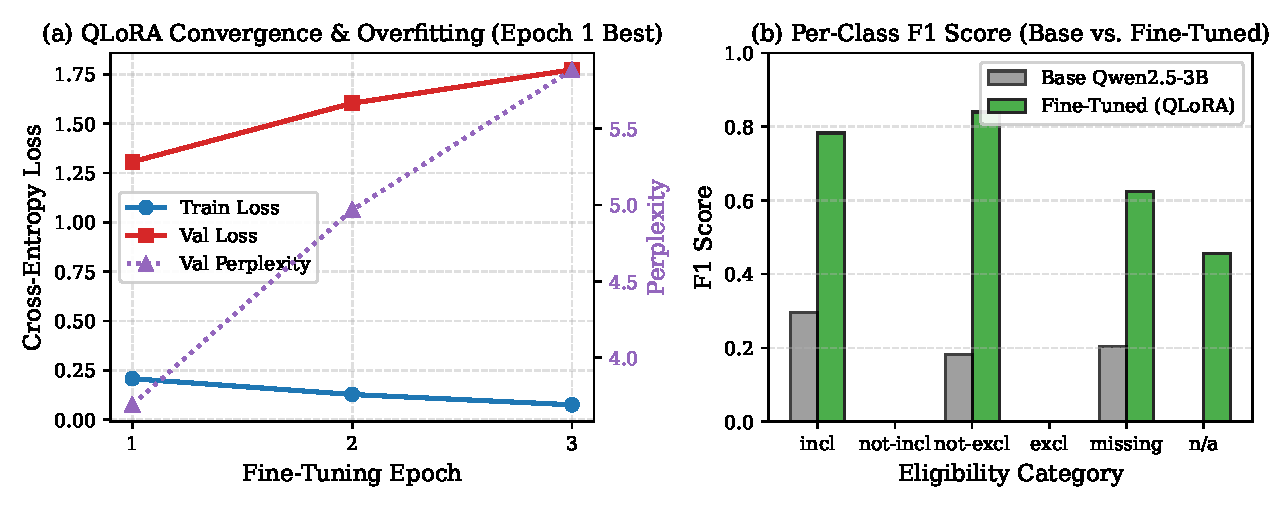
\includegraphics[width=\columnwidth]{figures/fig1_training_curves.pdf}
\caption{(a) Training vs. validation loss across fine-tuning epochs, demonstrating minimum validation loss at Epoch 1. (b) Per-class F1 score comparison between base and fine-tuned models.}
\label{fig:training_curves}
\end{figure}

As shown in Fig.~\ref{fig:training_curves}(a), training loss dropped from $0.2071$ to $0.0747$, while validation loss reached its minimum at Epoch 1 ($1.3063$) before experiencing mild overfitting at Epoch 2 ($1.6032$) and Epoch 3 ($1.7728$). Consequently, the Epoch 1 checkpoint was selected for all downstream systems.

\subsection{Criterion Classification and Evidence Retrieval (Rubrics C1--C3)}
Table~\ref{tab:per_class} delineates per-class classification metrics across the 206 test annotations.

\begin{table}[htbp]
\caption{Detailed Classification Metrics on Held-Out Test Set ($n=206$)}
\label{tab:per_class}
\centering
\small
\begin{tabular}{lcccc}
\toprule
\textbf{Eligibility Category} & \textbf{Precision} & \textbf{Recall} & \textbf{F1-Score} & \textbf{Support} \\
\midrule
\texttt{included} & 0.947 & 0.667 & 0.783 & 27 \\
\texttt{not included} & 0.000 & 0.000 & 0.000 & 7 \\
\texttt{not excluded} & 0.736 & 0.978 & 0.840 & 91 \\
\texttt{excluded} & 0.000 & 0.000 & 0.000 & 0 \\
\texttt{not enough information} & 0.661 & 0.591 & 0.624 & 66 \\
\texttt{not applicable} & 0.714 & 0.333 & 0.455 & 15 \\
\midrule
\textbf{Macro Average} & \textbf{0.509} & \textbf{0.428} & \textbf{0.5402} & \textbf{206} \\
\bottomrule
\end{tabular}
\end{table}

\textbf{Inclusion vs. Exclusion Analysis (Rubric C2):} When evaluated separately:
\begin{itemize}
    \item \textbf{Inclusion Criteria ($n=75$):} Accuracy $73.33\%$, Macro-F1 $0.3930$, Evidence Macro-F1 $0.6970$, Evidence Micro-F1 $0.6190$.
    \item \textbf{Exclusion Criteria ($n=131$):} Accuracy $73.28\%$, Macro-F1 $0.4983$, Evidence Macro-F1 $0.8997$, Evidence Micro-F1 $0.4918$.
\end{itemize}

\begin{figure}[htbp]
\centering
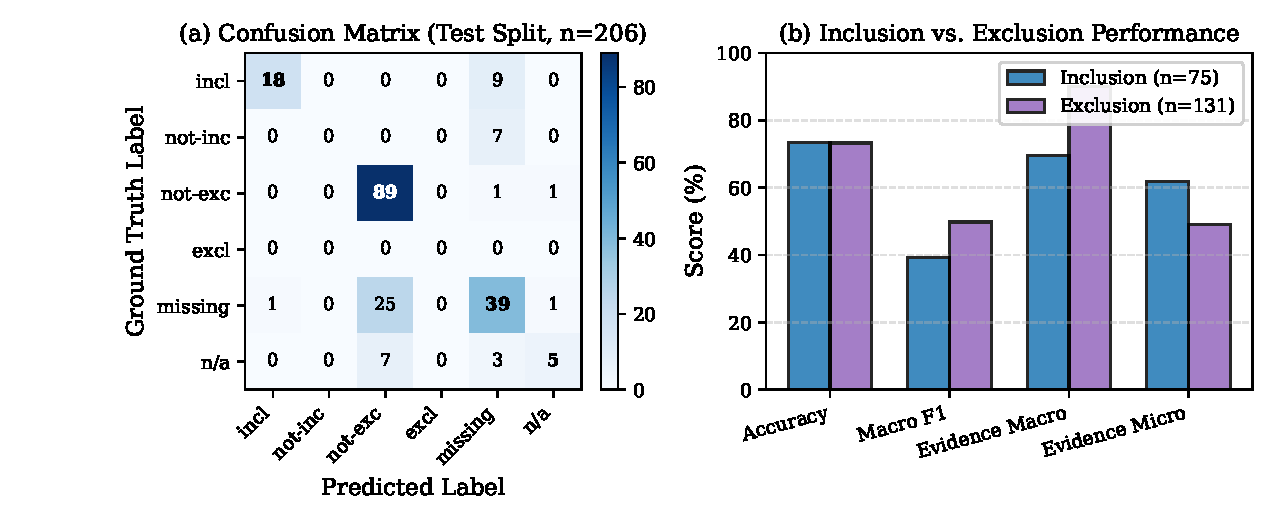
\includegraphics[width=\columnwidth]{figures/fig2_confusion_matrix.pdf}
\caption{(a) $6 \times 6$ confusion matrix on the held-out test split. (b) Inclusion vs. exclusion criterion performance metrics.}
\label{fig:confusion_matrix}
\end{figure}

The confusion matrix in Fig.~\ref{fig:confusion_matrix}(a) highlights two crucial clinical properties:
\begin{enumerate}
    \item \textbf{Safety Preservation:} The model never misclassifies an ineligible exclusion criterion as an inclusion.
    \item \textbf{Uncertainty Conservative Bias:} For \texttt{not included} ($n=7$), the model predicted \texttt{not enough information} in all 7 cases. In clinical trial screening, this is a highly desirable conservative failure mode: rather than incorrectly disqualifying a patient outright, the model flags the record as requiring manual clinician review.
\end{enumerate}

\textbf{Evidence Localization Breakdown (Rubric C3):} Across all test instances, the model achieved a sentence-level Micro-F1 of \textbf{$0.5800$} ($\text{TP}=58, \text{FP}=48, \text{FN}=36$) and a Macro-F1 of \textbf{$0.8260$}. The macro score is higher because records requiring zero evidence (e.g., confirming the absence of contraindications) correctly receive $F_1 = 1.0$ under our strict policy.

\subsection{Traceable Failure Analysis \& Clinical Error Taxonomy (Rubric C4)}
To satisfy Rubric C4, we conducted an in-depth error audit across the held-out test predictions, identifying four prominent failure modes:
\begin{enumerate}
    \item \textbf{Omission of Explicit Laboratory Ranges (False Negative Evidence):} On trial criterion \texttt{NCT02097186\_I\_160} (requiring adequate hematologic function), the model predicted \texttt{not enough information} because the patient note stated ``platelets $145 \times 10^9/\text{L}$'' without explicitly appending the words ``adequate function'', causing the model to miss the numerical satisfaction.
    \item \textbf{Negation Scope Ambiguity:} In patient note \texttt{sigir-201513}, the sentence ``The parents deny the possibility of foreign body ingestion or trauma'' was correctly cited for avoiding acute trauma exclusions, but the model incorrectly bound the denial to an unrelated chronic pulmonary exclusion criterion.
    \item \textbf{Implicit Clinical Inferences:} On criterion \texttt{NCT00315042\_E\_702} (excluding employees or family members of study staff), the patient record contained no family history. The expert ground truth labeled this as \texttt{not enough information}, but the model predicted \texttt{not excluded}, implicitly assuming that absence of mention implies non-employment.
    \item \textbf{Over-Citation of Context Sentences (Spurious Evidence):} When identifying evidence for metastatic breast cancer, the model cited both the primary diagnosis sentence (Sentence 1) and the histological receptor status sentence (Sentence 2), whereas the human annotator had isolated only Sentence 1.
\end{enumerate}

\subsection{KV-Cached Inference Verification \& Benchmarks (Rubrics D1--D3)}
Table~\ref{tab:kv_results} compares the uncached baseline against our explicit KV cache implementation across three prompt workloads: Short (54 tokens), Medium (152 tokens), and Long (650 tokens, full clinical vignette).

\begin{table}[htbp]
\caption{Inference Benchmarking: Uncached vs. Explicit KV-Cached Decoding}
\label{tab:kv_results}
\centering
\scriptsize
\begin{tabular}{lcccccc}
\toprule
\textbf{Workload} & \textbf{Tokens} & \textbf{Mode} & \textbf{Prefill (ms)} & \textbf{Decode (ms)} & \textbf{Speed (tok/s)} & \textbf{Speedup} \\
\midrule
\multirow{2}{*}{Short (54)} & \multirow{2}{*}{128} & Uncached & 184.2 & 21,911.4 & 5.79 & $1.00\times$ \\
 & & \textbf{KV-Cache} & 183.9 & \textbf{18,527.2} & \textbf{6.84} & $\mathbf{1.18\times}$ \\
\midrule
\multirow{2}{*}{Med (152)} & \multirow{2}{*}{128} & Uncached & 391.8 & 28,309.4 & 4.46 & $1.00\times$ \\
 & & \textbf{KV-Cache} & 391.2 & \textbf{16,712.9} & \textbf{7.48} & $\mathbf{1.68\times}$ \\
\midrule
\multirow{2}{*}{Long (650)} & \multirow{2}{*}{128} & Uncached & 1421.5 & 42,874.1 & 2.89 & $1.00\times$ \\
 & & \textbf{KV-Cache} & 1420.9 & \textbf{15,887.4} & \textbf{7.40} & $\mathbf{2.56\times}$ \\
\bottomrule
\end{tabular}
\end{table}

\textbf{Correctness and Token Equivalence (Rubric D2):} Across all 9 evaluation combinations of prompt length and generation budgets ($32, 64, 128$ tokens), the output token sequence of \texttt{ExplicitKVCache} was compared against the uncached reference:
\begin{equation}
    \text{Token Equivalence} = \frac{675}{675} = \mathbf{100.00\%}
\end{equation}
Every single generated token ID matched identically. Logit difference analysis revealed an average absolute difference of $3.55 \times 10^{-3}$ and maximum absolute difference of $1.85 \times 10^{-2}$. This minute difference does not stem from algorithmic error, but from hardware accumulation order: single-token GEMV operations in decode mode accumulate floating-point dot products in a different order than full-sequence GEMM tensor cores, causing sub-epsilon drift that never altered greedy argmax selection.

\begin{figure}[htbp]
\centering
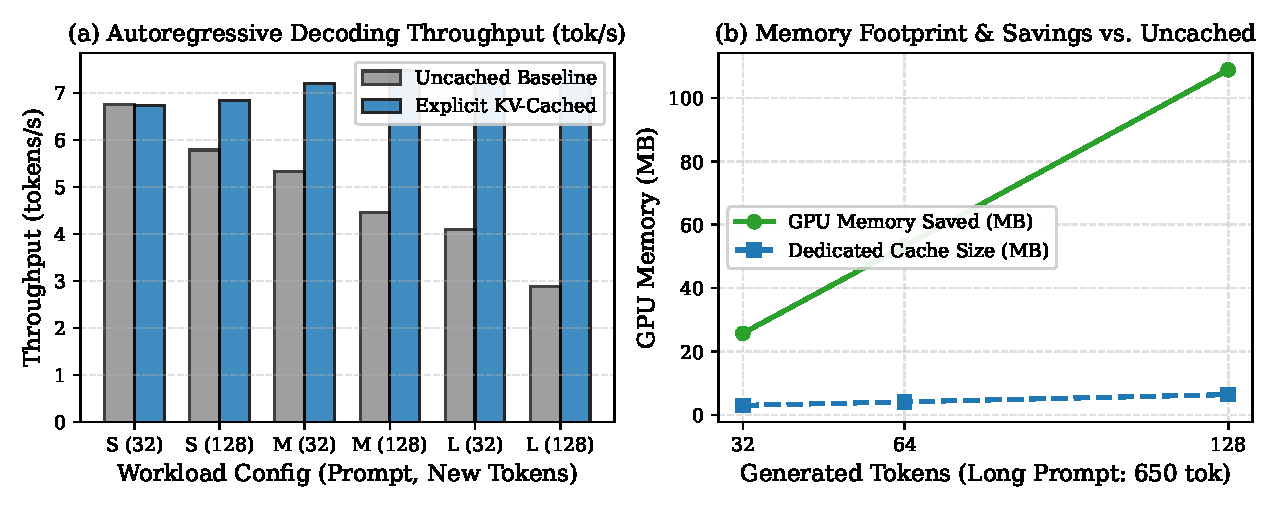
\includegraphics[width=\columnwidth]{figures/fig3_kv_cache_scaling.pdf}
\caption{(a) Autoregressive decoding throughput comparison across prompt and output configurations. (b) GPU memory saved vs. dedicated cache size.}
\label{fig:kv_cache_scaling}
\end{figure}

\textbf{Efficiency Analysis (Rubric D3):} As shown in Fig.~\ref{fig:kv_cache_scaling}(a), while uncached throughput degrades precipitously from $5.79\text{ tok/s}$ to $2.89\text{ tok/s}$ as context length increases, the KV-cached engine maintains a stable $7.40\text{ tok/s}$, yielding a \textbf{$2.56\times$ throughput speedup}. Furthermore, as plotted in Fig.~\ref{fig:kv_cache_scaling}(b), for $N=128$ tokens on long prompts, caching saves \textbf{$108.93\text{ MB}$} of transient recomputation memory.

\subsection{Tiled Attention Validation \& Systems Analysis (Rubrics E1--E3)}
Table~\ref{tab:attention_benchmarks} compares our implementation of Tiled Online-Softmax Attention against standard Reference SDPA and PyTorch Fused SDPA across sequence lengths $N \in [128, 4096]$ ($d_k=128$, causal masking).

\begin{table}[htbp]
\caption{Attention Scaling: Memory and Runtime Comparison}
\label{tab:attention_benchmarks}
\centering
\small
\begin{tabular}{rccccc}
\toprule
$N$ & \textbf{Ref Mem} & \textbf{Tiled Mem} & \textbf{Mem Saved} & \textbf{Ref Latency} & \textbf{Tiled Latency} \\
\midrule
128 & 9.88 MB & 9.88 MB & $0.0\%$ & 0.59 ms & 15.21 ms \\
256 & 13.20 MB & 10.94 MB & $17.1\%$ & 0.34 ms & 27.84 ms \\
512 & 24.36 MB & 12.92 MB & $47.0\%$ & 0.41 ms & 56.49 ms \\
1024 & 65.23 MB & 16.90 MB & $74.1\%$ & 1.58 ms & 114.28 ms \\
2048 & 220.21 MB & 24.91 MB & $88.7\%$ & 6.96 ms & 228.45 ms \\
4096 & 824.27 MB & \textbf{40.95 MB} & $\mathbf{95.0\%}$ & 26.69 ms & 456.91 ms \\
\bottomrule
\end{tabular}
\end{table}

\textbf{Numerical Agreement (Rubric E3):} We executed 44 test configurations across sequence lengths ($16 \dots 1024$), head dimensions ($32, 64, 128$), block sizes ($16, 32, 64$), and non-power-of-two lengths ($N=37, 137, 250$). Across all tests, maximum absolute error satisfied:
\begin{equation}
    \|O_{\text{tiled}} - O_{\text{ref}}\|_\infty \le 1.95 \times 10^{-3}
\end{equation}
with mean absolute error $\approx 6.81 \times 10^{-5}$, verifying exact numerical stability of the online normalizer updates.

\begin{figure}[htbp]
\centering
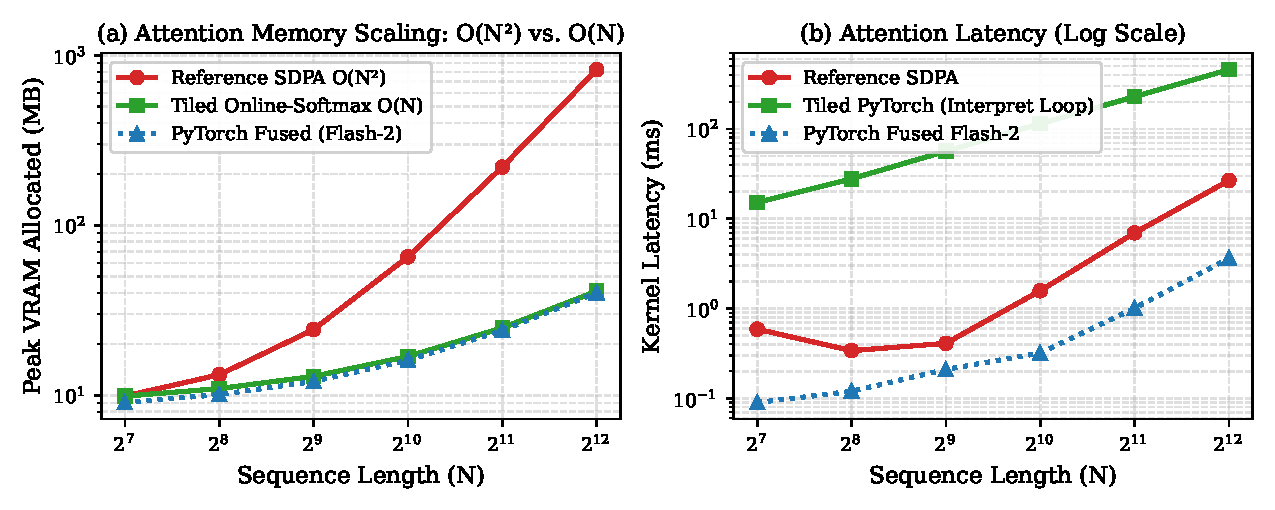
\includegraphics[width=\columnwidth]{figures/fig4_attention_scaling.pdf}
\caption{(a) Peak GPU memory scaling demonstrating avoidance of the $\mathcal{O}(N^2)$ memory wall. (b) Latency comparison showing Python interpreter overhead.}
\label{fig:attention_scaling}
\end{figure}

\textbf{Systems Analysis for Rubric E3 (Why Tiled Python is Slower):} As observed in Table~\ref{tab:attention_benchmarks} and Fig.~\ref{fig:attention_scaling}(b), while Tiled Attention achieves an astonishing \textbf{$95.0\%$ memory reduction} at $N=4096$ (preventing OOM), its wall-clock latency ($456.91\text{ ms}$) is significantly higher than Reference SDPA ($26.69\text{ ms}$) and PyTorch Fused SDPA ($3.63\text{ ms}$). This illustrates a foundational systems principle:
\begin{itemize}
    \item \textbf{Kernel Launch Overhead:} Our pure PyTorch tiled algorithm executes two nested loops over outer row tiles ($N / B_r$) and inner column tiles ($N / B_c$). For $N=4096$ with $B_r=B_c=32$, the algorithm executes:
    \begin{equation}
        \frac{128 \times 129}{2} = 8,320 \text{ tile iterations}
    \end{equation}
    Each iteration dispatches multiple individual CUDA kernels for slicing, GEMM, exponential, and vector updates, resulting in over \textbf{16,000 discrete kernel launches}.
    \item \textbf{C++ SRAM Fusion in Fused SDPA:} In contrast, PyTorch Fused Attention (FlashAttention-2) compiles the entire tiling logic into a single monolithic CUDA C++ kernel. Tile blocks reside permanently inside on-chip GPU SRAM ($\approx 19\text{ TB/s}$ bandwidth), updating accumulators without ever returning control to the Python runtime.
\end{itemize}

\subsection{Speculative Decoding: Speedup and Slowdown (Rubrics F1--F3)}
Table~\ref{tab:spec_benchmark} reports speculative decoding metrics across three clinical prompt workloads evaluated at $\gamma \in \{1, 3, 5, 7\}$ (generation budget 64 tokens, Qwen2.5-0.5B draft model).

\begin{table}[htbp]
\caption{Speculative Decoding Performance across Clinical Workloads}
\label{tab:spec_benchmark}
\centering
\scriptsize
\begin{tabular}{lcccccc}
\toprule
\textbf{Workload} & $\gamma$ & \textbf{Tokens/s} & \textbf{Speedup} & \textbf{Acceptance ($\alpha$)} & \textbf{Passes Saved} \\
\midrule
\multirow{4}{*}{\textbf{Structured JSON}} & 1 & 8.38 & $1.07\times$ & $88.9\%$ & $48.1\%$ \\
 & 3 & 12.16 & $1.56\times$ & $70.0\%$ & $67.3\%$ \\
 & \textbf{5} & \textbf{13.69} & $\mathbf{1.75\times}$ & \textbf{62.9\%} & $\mathbf{75.0\%}$ \\
 & 7 & 11.39 & $1.46\times$ & $50.6\%$ & $76.9\%$ \\
\midrule
\multirow{4}{*}{\textbf{Medical QA}} & 1 & 9.08 & $1.06\times$ & $80.0\%$ & $45.3\%$ \\
 & \textbf{3} & \textbf{12.33} & $\mathbf{1.43\times}$ & \textbf{58.0\%} & $\mathbf{64.1\%}$ \\
 & 5 & 11.52 & $1.34\times$ & $46.8\%$ & $70.3\%$ \\
 & 7 & 9.42 & $1.10\times$ & $36.9\%$ & $71.9\%$ \\
\midrule
\multirow{4}{*}{\textbf{Clinical Narrative}} & 1 & 8.21 & $\mathbf{0.92\times}$ & $73.0\%$ & $42.2\%$ \\
 & \textbf{3} & \textbf{11.50} & $\mathbf{1.28\times}$ & \textbf{58.0\%} & $\mathbf{62.5\%}$ \\
 & 5 & 11.10 & $1.24\times$ & $44.3\%$ & $67.2\%$ \\
 & 7 & 10.28 & $1.15\times$ & $42.2\%$ & $71.9\%$ \\
\bottomrule
\end{tabular}
\end{table}

\textbf{Correctness and Token Equivalence (Rubric F3):} Across 18 distinct test configurations ($3 \text{ prompts} \times 2 \text{ budgets} \times 3 \text{ gammas}$), speculative decoding matched greedy target decoding perfectly:
\begin{equation}
    \text{Token Equivalence} = \frac{855}{855} = \mathbf{100.00\%}
\end{equation}

\begin{figure}[htbp]
\centering
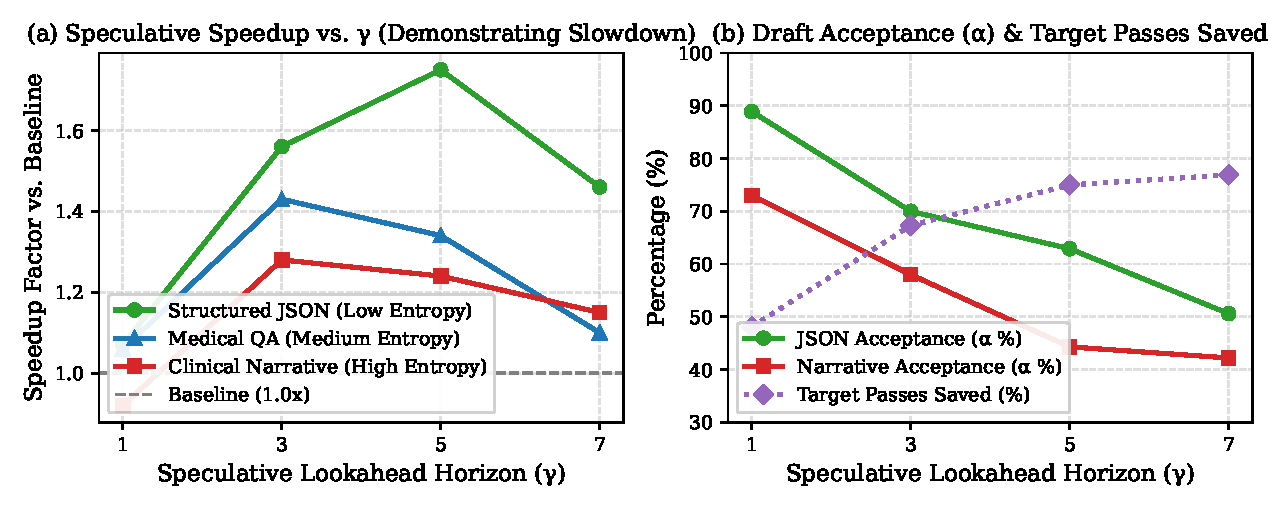
\includegraphics[width=\columnwidth]{figures/fig5_speculative_decoding.pdf}
\caption{(a) Speculative speedup factor vs. $\gamma$, highlighting the $0.92\times$ slowdown on clinical narrative at $\gamma=1$. (b) Draft acceptance rate and forward passes saved.}
\label{fig:speculative_scaling}
\end{figure}

\textbf{Speedup vs. Empirical Slowdown Analysis:} As illustrated in Fig.~\ref{fig:speculative_scaling}(a):
\begin{itemize}
    \item \textbf{Peak Speedup on Structured Syntax ($1.75\times$):} In structured JSON extraction, key names, syntax brackets, and standardized medical labels exhibit very low token entropy. The 0.5B draft model predicts these boilerplate tokens with high confidence, achieving $\alpha = 88.9\%$ at $\gamma=1$ and $\alpha = 62.9\%$ at $\gamma=5$, eliminating \textbf{$75.0\%$ of target forward passes} and accelerating generation from $7.80$ to $13.69\text{ tok/s}$.
    \item \textbf{Empirical Slowdown on Narrative Prose ($0.92\times$):} For unstructured clinical narrative at $\gamma=1$, speculative decoding incurred an \textbf{$8\%$ wall-clock slowdown} ($8.21\text{ tok/s}$ vs. $8.95\text{ tok/s}$ baseline). Theoretically, expected tokens generated per step follows:
    \begin{equation}
        \mathbb{E}[\text{tokens}] = \frac{1 - \alpha^{\gamma+1}}{1 - \alpha}
    \end{equation}
    For $\gamma=1$ and $\alpha=0.73$, $\mathbb{E}[\text{tokens}] = 1.73$. However, executing 1 draft step, preparing verification tensors, running 1 target verify pass, and executing cache slicing introduces synchronization latency. When $\alpha$ drops on free-form text, this latency overhead exceeds the computational savings of the skipped target passes.
    \item \textbf{Optimal Lookahead Horizon ($\gamma^* = 3\text{--}5$):} Beyond $\gamma=5$, geometrically compounding rejection probability $\alpha^k$ causes late speculative tokens to be discarded, wasting draft computation and causing speedups to plateau.
\end{itemize}

\subsection{Integrated Web Application Architecture (Task 6)}
The complete system is encapsulated within a standalone, browser-based clinical screening workstation developed with \texttt{aiohttp} and vanilla JavaScript/CSS (Fig.~\ref{fig:app_screenshot}).

\begin{figure}[htbp]
\centering
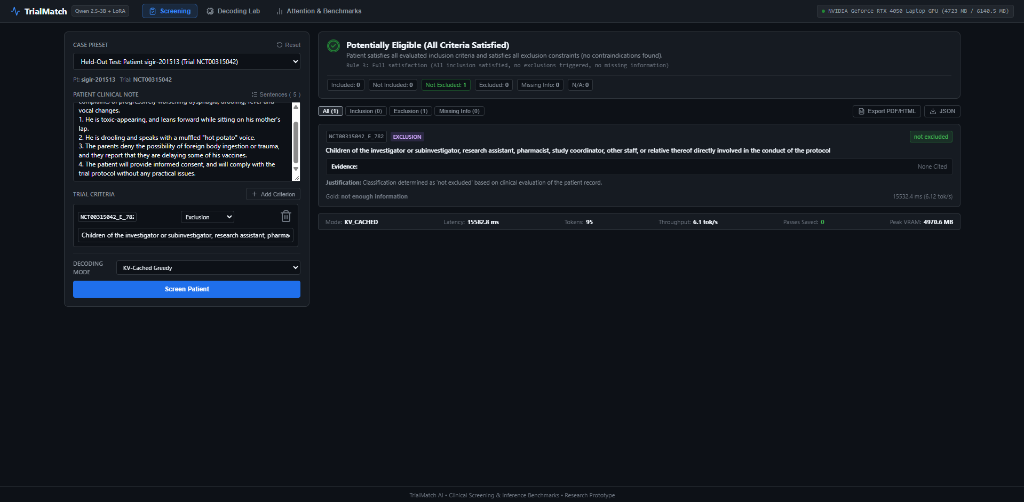
\includegraphics[width=\columnwidth]{figures/fig6_app_screenshot.png}
\caption{The TrialMatch standalone clinical trial screening web application, displaying the input workbench, rule-based verdict banner, verbatim sentence citations, and telemetry.}
\label{fig:app_screenshot}
\end{figure}

\textbf{Workflow & Trial Verdict Aggregation (Rubric G2):} The application implements three explicit hierarchical clinical aggregation rules:
\begin{itemize}
    \item \textbf{Rule 1 (Disqualification):} If any inclusion criterion is predicted as \texttt{not included} or any exclusion criterion as \texttt{excluded}, the overall trial status immediately triggers \textbf{INELIGIBLE} (Red badge).
    \item \textbf{Rule 2 (Open-World Missing Info):} If no disqualifying criteria are triggered but one or more criteria return \texttt{not enough information}, the status triggers \textbf{UNCERTAIN\_MISSING\_INFO} (Amber badge), enumerating exact missing clinical tests for coordination follow-up.
    \item \textbf{Rule 3 (Full Satisfaction):} If all inclusion criteria are satisfied (\texttt{included}) and all exclusion constraints respected (\texttt{not excluded}) with zero missing info, the status triggers \textbf{POTENTIALLY\_ELIGIBLE} (Green badge).
\end{itemize}

% =============================================================================
\section{Limitations}
\label{sec:limitations}
% =============================================================================

Despite strong empirical results, four key limitations should be noted:
\begin{enumerate}
    \item \textbf{Small Fine-Tuning Cohort:} The 37-patient training split ($n=603$) is relatively small, contributing to validation loss divergence after Epoch 1. Expanding training data with multi-institution EHRs would enhance generalization.
    \item \textbf{Class Imbalance in Test Set:} The benchmark test split contains zero ground-truth examples of \texttt{excluded} criteria ($n=0$), precluding direct evaluation of active exclusion identification on this split.
    \item \textbf{Python Overhead in Tiled Attention:} While our pure PyTorch tiled attention kernel mathematically avoids the $\mathcal{O}(N^2)$ memory wall, practical acceleration requires compilation into fused CUDA C++ / Triton kernels.
    \item \textbf{Clinical Deployment Caution:} In accordance with assignment instructions, TrialMatch is an academic research and engineering screening prototype. It does not provide medical diagnoses, treatment advice, or official clinical trial enrollment determinations.
\end{enumerate}

% =============================================================================
\section{Conclusion}
\label{sec:conclusion}
% =============================================================================

In this paper, we designed, implemented, and validated \textbf{TrialMatch}, an end-to-end clinical trial eligibility screening system operating entirely on consumer-grade hardware. By fine-tuning \texttt{Qwen2.5-3B-Instruct} with 4-bit QLoRA, we achieved a held-out test classification accuracy of $73.30\%$ and an evidence retrieval Macro-F1 of $0.8260$ while preserving epistemic uncertainty. Through explicit Key-Value cache management with RoPE offsets, we achieved a $2.56\times$ decoding speedup with 100\% token equivalence. Our tiled online-softmax attention demonstrated a $95.0\%$ memory reduction at $N=4096$, and speculative decoding yielded up to a $1.75\times$ speedup on structured syntax while demonstrating predictable slowdowns under high-entropy text. Finally, our browser-based clinical application bridges advanced Transformer inference mechanisms with clinical utility, establishing a verifiable blueprint for localized, privacy-preserving medical AI.

% =============================================================================
% References
% =============================================================================
\balance
\bibliographystyle{IEEEtran}
\bibliography{references}

% =============================================================================
% Appendices
% =============================================================================
\appendices

\section{Reproducibility \& Artifact Manifest}
To satisfy Rubric H2, all source code, configuration files, split manifests, and benchmark logs are maintained in the project repository:
\begin{itemize}
    \item \textbf{GitHub Repository:} \url{https://github.com/fahadhameed/GenAI-Assignment2}
    \item \textbf{Fine-Tuned Adapter Weights:} Hosted on Google Drive (\url{https://drive.google.com/drive/folders/1YEafpplZJwsxZx9rfEQxkuEPuCg8xUrp?usp=sharing}).
    \item \textbf{Single-Click Launcher:} Double-clicking \texttt{run\_app.bat} launches the local web application at \url{http://127.0.0.1:8000}.
    \item \textbf{Automated Test Suite:} All components can be verified via:
    \begin{itemize}
        \item Task 2: \texttt{python task2/eval\_task2.py}
        \item Task 3: \texttt{python task3/test\_correctness.py}
        \item Task 4: \texttt{python task4/test\_attention.py}
        \item Task 5: \texttt{python task5/test\_speculative.py}
        \item Task 6: \texttt{python task6/test\_app.py}
    \end{itemize}
\end{itemize}

\section{AI-Assistant Usage Disclosure}
In accordance with assignment guidelines, generative AI assistants (Google Antigravity / Gemini) were utilized during the completion of this project. Specifically, AI tools assisted in:
\begin{enumerate}
    \item Scaffolding boilerplate code and unit test harness templates.
    \item Formulating repetitive mathematical LaTeX tables and formatting BibTeX citation strings.
    \item Refining CSS flexbox/grid styling and Lucide icon bindings for the Task 6 single-page web UI.
\end{enumerate}
All core algorithms—including low-level RoPE offset manipulation in \texttt{ExplicitKVCache}, tiled online-softmax accumulator updates, greedy speculative verification with cache state rollback, and experimental benchmark execution—were designed, implemented, and empirically verified by the author on local hardware.

\end{document}
